\section{Architecture Integration}

\subsection{Model Support}

\begin{table}[H]
\centering
\small
\begin{tabular}{lllll}
\toprule
\textbf{Model} & \textbf{Attention path} & \textbf{Nested?} & \textbf{RoPE?} & \textbf{GQA?} \\
\midrule
DistilBERT & \texttt{layer[i].attention} & No & No & No \\
RoBERTa & \texttt{layer[i].attention.self} & Yes & No & No \\
GPT-2 & \texttt{h[i].attn} & No & No & No \\
Qwen3.5 & \texttt{layers[i].self\_attn} & No & Yes & Yes \\
PyTorch MHA & Any & Varies & Varies & Varies \\
\bottomrule
\end{tabular}
\end{table}

\subsection{Weight Transfer Patterns}

The \texttt{copy\_weights} procedure handles five patterns:

\subsubsection{Pattern 0: PyTorch `MultiheadAttention`}

\begin{lstlisting}
w\_q, w\_k, w\_v = src.in\_proj\_weight.chunk(3, dim=0)
b\_q, b\_k, b\_v = src.in\_proj\_bias.chunk(3, dim=0)
w\_o = src.out\_proj.weight
\end{lstlisting}

\subsubsection{Pattern 1: GPT-2 Conv1D}

\begin{lstlisting}
c\_w = src.c\_attn.weight.t()  # transpose
q\_w, k\_w, v\_w = c\_w.chunk(3, dim=0)
w\_o = src.c\_proj.weight.t()
\end{lstlisting}

\subsubsection{Pattern 2: RoBERTa Nested}

\begin{lstlisting}
w\_q = src.self.query.weight
w\_k = src.self.key.weight
w\_v = src.self.value.weight
w\_o = src.output.dense.weight
\end{lstlisting}

\subsubsection{Pattern 3: Qwen / LLaMA}

\begin{lstlisting}
w\_q = src.q\_proj.weight
w\_k = src.k\_proj.weight
w\_v = src.v\_proj.weight
w\_o = src.o\_proj.weight
\end{lstlisting}

\subsubsection{Pattern 4: DistilBERT}

\begin{lstlisting}
w\_q = src.q\_lin.weight
w\_k = src.k\_lin.weight
w\_v = src.v\_lin.weight
w\_o = src.out\_lin.weight
\end{lstlisting}

\subsection{What Gets Copied}

HGRN2Layer uses only \textbf{V} and \textbf{O} projections from the pretrained attention:

\begin{table}[H]
\centering
\small
\begin{tabular}{ll}
\toprule
\textbf{Pretrained projection} & \textbf{HGRN2Layer target} \\
\midrule
Q & (unused) \\
K & (unused) \\
V & \texttt{v\_proj} \\
O & \texttt{out\_proj} \\
\bottomrule
\end{tabular}
\end{table}

The Q and K projections are discarded because HGRN2Layer has no query-key 
mechanism.

\subsection{Nested Encoder Handling}

For RoBERTa and BERT, \texttt{is\_nested\_encoder = True}. The injection procedure 
replaces \texttt{layer.attention.self} with the HGRN2Layer and sets 
\texttt{layer.attention.output.dense = nn.Identity()}. This ensures the output 
projection is not applied twice.

\subsection{Injection Algorithm}

\textbf{Algorithm 2:} Inject HGRN2Layer into a model
\begin{lstlisting}
Input:  model M, config c
Output: M with attention replaced

1: layer\_list $\leftarrow$ find\_transformer\_layers(M)
2: for i, layer in enumerate(layer\_list) do
3:     if not has\_attention(layer): continue
4:     src $\leftarrow$ get\_attention(layer)
5:     new $\leftarrow$ HGRN2Layer(c, old\_attn=src, ...)
6:     if is\_nested(layer):
7:         layer.attention.self = new
8:         layer.attention.output.dense = nn.Identity()
9:     else:
10:        replace\_attention(layer, new)
11: end for
12: return M
\end{lstlisting}

\subsection{Cross-Attention}

Cross-attention is \textbf{not supported}. If \texttt{encoder\_hidden\_states} is provided, 
we raise \texttt{NotImplementedError}.

\subsection{Failure Modes}

\begin{table}[H]
\centering
\small
\begin{tabular}{lll}
\toprule
\textbf{Failure} & \textbf{Detection} & \textbf{Response} \\
\midrule
V/O not extractable & \texttt{copy\_weights} fails & Log warning, keep random \\
Nested detection wrong & \texttt{is\_nested\_encoder} mis-set & Degraded output \\
OOM in scan & GPU memory exhausted & Reduce batch or chunk size \\
Cross-attention call & \texttt{encoder\_hidden\_states} not None & Raise \\
\bottomrule
\end{tabular}
\end{table}

\subsection{Double-Injection Guard}

The injection function does not check for double injection in this module 
version, since the \texttt{HGRN2Layer} class name match is uncommon. However, we 
recommend adding a check if re-injection is a concern.

\subsection{Registry}

\begin{lstlisting}
@ATTENTION\_REGISTRY.register("hgrn2\_layer")
@ATTENTION\_REGISTRY.register("hgrn2")
class HGRN2Layer(BaseAttention):
    ...
\end{lstlisting}

\subsection{Design Notes}

\textbf{Bidirectional by default for encoders.} The scan runs forward and backward 
and sums the results, giving each token access to both past and future context.

\textbf{Causal for decoders.} Only the forward scan is used.

\textbf{Chunk size = 32.} Chosen as a balance between parallelism (more chunks = 
more parallel work) and memory (larger chunks = larger intra-chunk matrices).
\begin{lstlisting}

---
\end{lstlisting}

\begin{figure}[H]
\centering
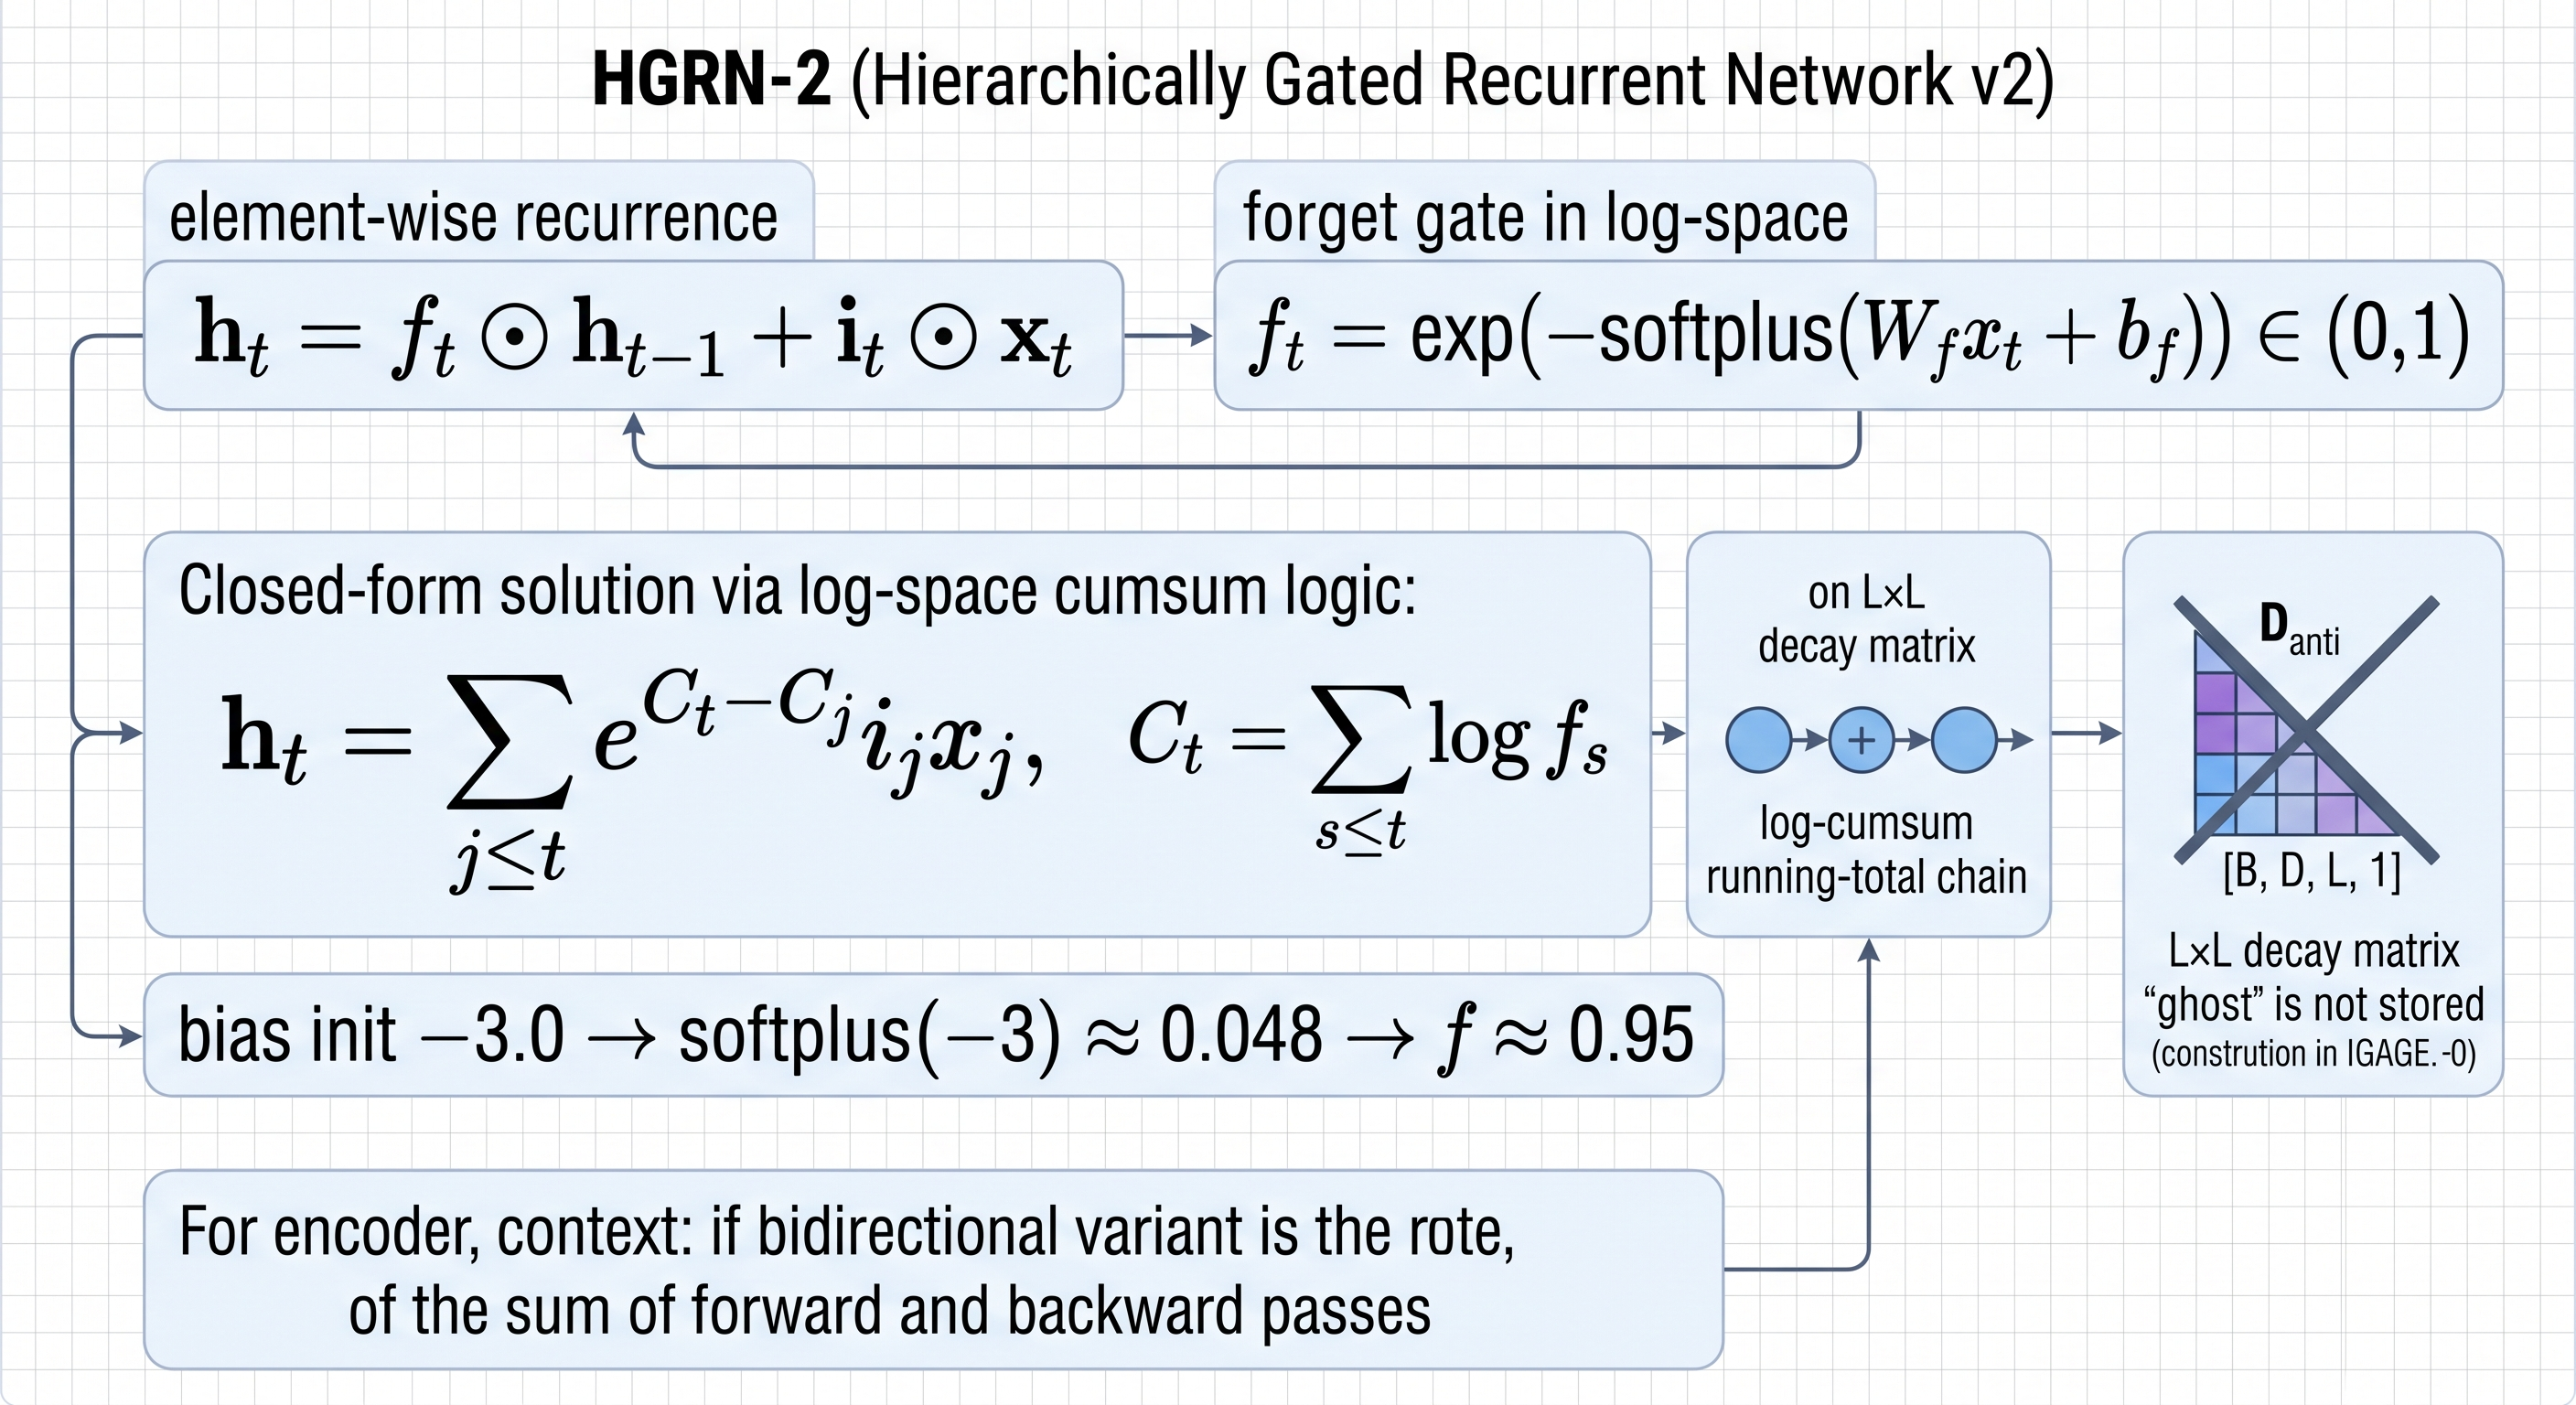
\includegraphics[width=\linewidth]{figures/architecture.jpeg}
\caption{High-level architectural diagram of hgrn2\_layer.}
\label{fig:arch_hgrn2-layer}
\end{figure}

